\documentclass[a4paper,12pt]{article}
\usepackage{geometry}
 \geometry{
 a4paper,
 total={210mm,297mm},
 left=20mm,
 right=20mm,
 bottom=20mm,
 top=20mm,
 }
\usepackage[english]{babel}
\usepackage[T1]{fontenc}
\usepackage{xcolor}
\usepackage[utf8]{inputenc}
\usepackage{lmodern}
\usepackage{microtype}
\usepackage{graphicx}
\usepackage{caption} 
\usepackage{titling}
\usepackage[colorlinks=true,linkcolor=black,urlcolor=blue]{hyperref}
\usepackage{indentfirst}
\usepackage{siunitx}
\usepackage{amsmath}
\usepackage{multicol}
\usepackage{enumitem}
\usepackage{listings}
\usepackage{matlab-prettifier}





\title{Signal and Systems II Project \\ [1ex]\large Processing motion signals from a PTZ camera  }
\author{Ulysse MERAD\and Ruben LEGRANDJACQUES \and \\Fabrice LIN \and Anwar AL-BITAR}

\date{December 12\textsuperscript{th}, 2023} 

\begin{document}

\begin{titlepage}
  \centering
  \vspace{3cm}
  \Huge{\color{blue}\textbf{CT.2306 : Signal  \& Systems II }}\\
  \vspace{1cm}
  \Huge{\underline{\textbf{Project Report:}}}\\
  \vspace{0.5cm}
  \Large{ \underline{Processing motion signals from a PTZ camera}} \\
  \vspace{1cm}
  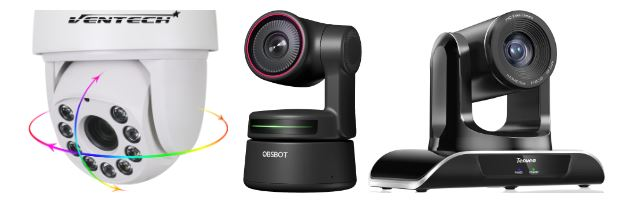
\includegraphics[scale=1]{camera.jpg}\\
  \vspace{0.5cm}
  Ulysse MERAD, Ruben LEGRANDJACQUES, \\ [0.5ex] Fabrice LIN, Anwar AL-BITAR \\
  \vspace{1.5cm}
  \large{\textit {Under the supervision of A.BAHLOUL and I.AYAJI}} \\
  \vspace{1.5cm}
  \thedate \\
  \vspace{2cm}
  
\includegraphics[scale=0.7]{Isep.jpg}\\
  
\end{titlepage}

\begin{abstract}
  Sum-up of the project
\end{abstract}

\tableofcontents
\setlength{\parskip}{10pt}

\newpage


\section{Data Visualization}
\begin{enumerate}[label={\color{blue}\arabic*)}]

\item \emph{Loading data}

We first use \textit{load('data-proj.mat')} to load variables from data file. Then using \textit{whos} we can list all variables. We have their name and size.
Here is the result : 


\begin{lstlisting}[style=Matlab-editor,language=Matlab, caption= Loaded variables, captionpos=b]
  >> whos
Name       Size                Bytes  Class     

omega      1x20001            160008  double              
t          1x20001            160008  double 
  
\end{lstlisting}


\item \emph{Plotting the data}

We can not use the signal as it is. Graphically it is impossible to analyze. Either it is too noisy or the window is too large in order to see enough details of the signal. This is a continous (analog) signal. Electronic control devices requires digital signals.
\begin{multicols}{2}
\begin{center}
  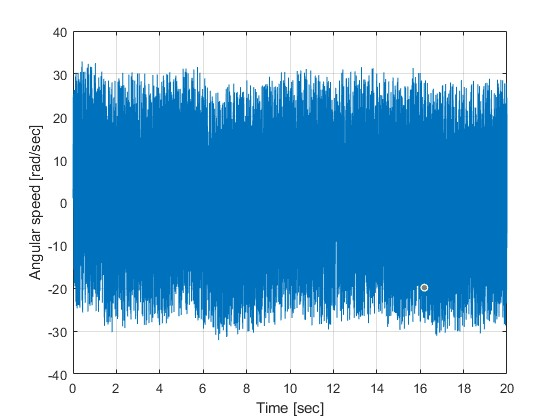
\includegraphics[scale=0.35]{Figures/q2.jpg}
  \captionof{figure}{Angular speed as a function of time}
  \label{F2}
\end{center}
\columnbreak

\begin{lstlisting}[style=Matlab-editor,language=Matlab, caption={Code for Figure 2}, captionpos=b, basicstyle=\small\ttfamily]
  %% Plot of angular speed
  fig=1
  figure(fig)
  plot()
  grid on 
  xlabel('Time [sec]')
  ylabel('Angular speed [rad/sec]')
  \end{lstlisting}
\end{multicols}
\end{enumerate}

\section{Analog Filtering}
\begin{enumerate}[label={\color{blue}\arabic*)}]
  \setcounter{enumi}{2}
  \item \emph{Sampling period \(T_{e_1}\)}
  
  We deduce the Sampling period \(T_{e_1}\) with the subtraction of two consecutive values of \(t\). Also, graphically we observe the run between 2 straight line in the signal if we zoom. \(\mathbf{T_{e_1}=1.10^{-3} sec}\) 
  \begin{multicols}{2}
    \begin{center}
      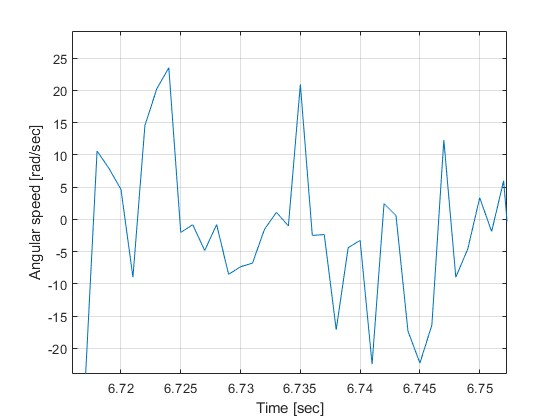
\includegraphics[scale=0.3]{Figures/q3.jpg}
      \captionof{figure}{Same signal with zoom}
      \label{F2}
    \end{center}
    \columnbreak
    
    \begin{lstlisting}[style=Matlab-editor,language=Matlab, caption={Code for Figure 2}, captionpos=b, basicstyle=\small\ttfamily]
      %% Sampling period
      Te1=t(5)-t(4)

      >>Te1 =

      1.0000e-03
      \end{lstlisting}
    \end{multicols}
  \item \emph{DFT}
  
Using code from workshop 5 and Help Project, we obtain this plot.
\begin{multicols}{2}
\begin{flushleft}
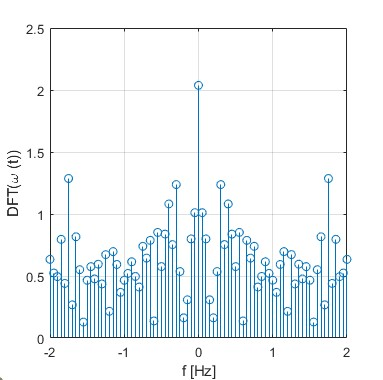
\includegraphics[scale=0.6]{Figures/q4.jpg}
\captionof{figure}{DFT plot of \(\omega(t)\)}
\label{F3}
\end{flushleft}
\columnbreak
\begin{lstlisting}[style=Matlab-editor,language=Matlab, caption={Code for Figure 3}, captionpos=b, basicstyle=\small\ttfamily]
Te2= 0.05;%sampling period 
Fe2=1/Te2;%sampling frequency
Tf=t(end);%singal duration
N=Tf/Te2;%number of samples 
%(N=Duration/sampling period)
%frequency vector
f1=-Fe2*(N/2-1)/N:Fe2/N:0;
f2=Fe2/N:Fe2/N:(N/2)*Fe2/N;
f=[f2,f1];
O= zeros(1,N);
for m=1:N
  for k=1:N
    O(m)=O(m)+omega(k)*exp(-j*2*pi*m*k/N);
  end
end
figure(fig+1);
stem(f,abs(O)/N)
grid on
xlim([-2,2])
xlabel('f [Hz]')
ylabel('DFT(\omega (t))')
\end{lstlisting}
\end{multicols}
      
    
  \item \emph{Maximal Frequency \(F_{max}\) of the signal}
  
  \colorbox{yellow}{I don't know yet exactly what to do maybe the maximum frequency \(F_e = 2 Hz\)}.
  \item \emph{ First order low-pass analog filter of a unit gain}
  
  We first create a unit gain low-pass filter with a cutoff frequency \(f_c = 2 Hz\) \textbf{using Matlab.}
  \begin{multicols}{2}
\begin{flushleft}
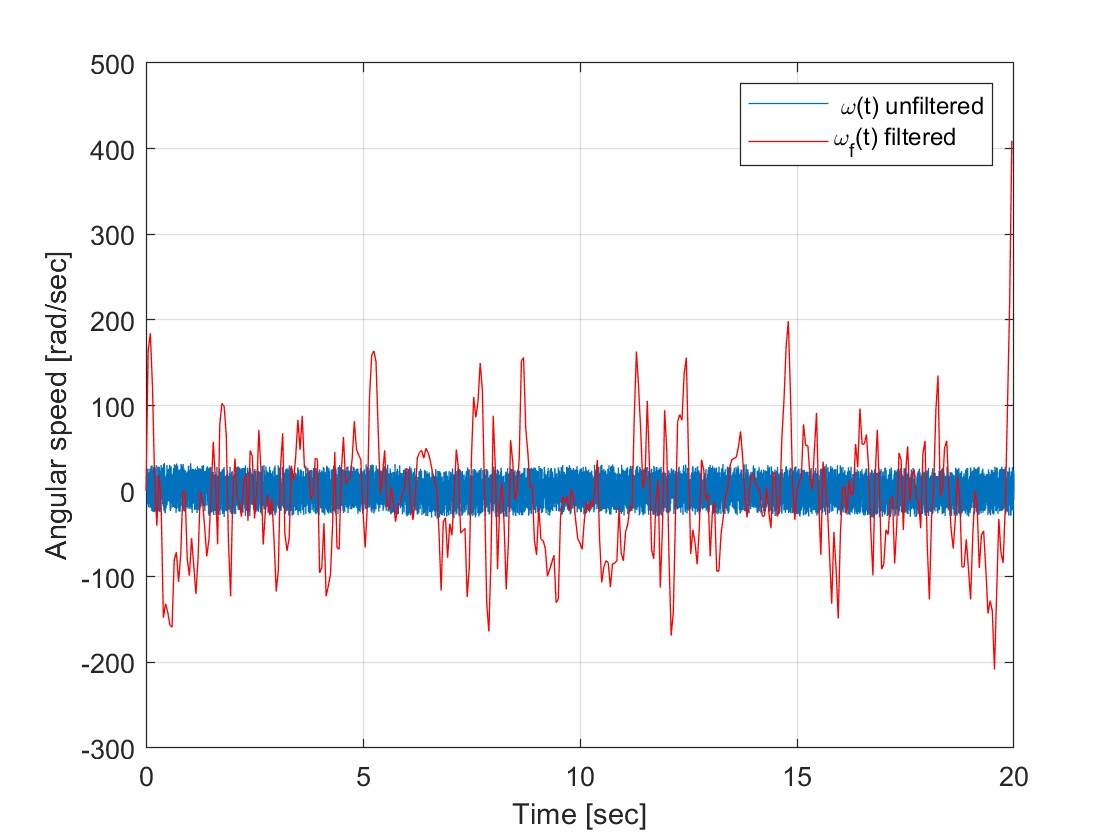
\includegraphics[scale=0.2]{Figures/q6a.jpg}
\captionof{figure}{Plot of unfiltered and filtered \(\omega\) signal} 
\label{F3}
\end{flushleft}
\columnbreak
\begin{lstlisting}[style=Matlab-editor,language=Matlab, caption={Code for Figure 4}, captionpos=b, basicstyle=\small\ttfamily]
%create the new time vector 
t1=0:Te2:t(end)-Te2;
%% filter design
fc1=2;
H1=tf(1,[1/(2*pi*fc1)  1]);
Of=lsim(H1,O,t1);
%% plot of filtered signal
figure(1);
plot(t1,Of,'r')
grid on
legend(' \omega(t) unfiltered','\omega_{f}(t) filtered')
\end{lstlisting}
\end{multicols}
We may notice that we observe on the red filtered signal that its amplitude is bigger. We do not know exactly why. Bode diagram show a magnnitude near 0 from low frequencies.
  \item \emph{question subject}
\end{enumerate}

\section{Sampling}
\begin{enumerate}[label={\color{blue}\arabic*)}]
  \setcounter{enumi}{7}
  \item \emph{question subject}
  \item \emph{question subject}
  \item \emph{question subject}
  \item \emph{question subject}
  \item \emph{question subject}
\end{enumerate}

\section{Angular position and acceleration}
\begin{enumerate}[label={\color{blue}\arabic*)}]
  \setcounter{enumi}{12}
  \item \emph{question subject}
  \item \emph{question subject}
  \item \emph{question subject}
\end{enumerate}

\section{Digital filtering}
\begin{enumerate}[label={\color{blue}\arabic*)}]
  \setcounter{enumi}{15}
  \item \emph{question subject}
  \item \emph{question subject}
  \item \emph{question subject}
\end{enumerate}




\end{document}